%!TEX root = linear-algebra.tex
\stepcounter{lecture}
\setcounter{lecture}{3}

\sektion{Forces}
\subsektion{Gravity}
\subsektion{Contraint Forces}
\subsektion{Friction}
\subsektion{Drag Force}
\lecturemarker{15}{22 Oct}

Example of a force that depends on the velocity of an object. 

Motion of bodies through fluid. 
\vspace*{100pt}

Fluid has: $\rho$: density and $\eta$: viscosity

To move through the fluid, the body exerts a force on the fluid: $\vec{F}_{FB}$

By Newton's III Law
\[\vec{F}_{BF} = -\vec{F}_{FB}\]
The drag force \[\vec{F}_D = (\vec{F}_{BF}\cdot \hat{v})\hat{v}\]

In general to find $\vec{F}_{D}$ is a challenging problem!

To find $\vec{u}$ we need to solve the Navier-Stokes Equations. From $\vec{u}$ we can obtain $\vec{F}_D$. 

Fortunately this calculation can be done for two limiting cases; at low and at high speeds:

\subsubsektion{Low Speeds}
At low speeds $|\vec{v}| << 1$, then 
\[\vec{F}_D = -C_D\vec{v}\]
Where $C_D$ is the \emph{drag co-efficient}

\begin{itemize}
\item This depends linearly on $\vec{v}$.
\item Always opposite the direction of motion
\item For a sphere $C_D = 6\pi R\eta$
\item $C_D$ depends on (i) the size of the object, (ii) the viscosity of the fluid
\end{itemize}
If $\vec{u} \neq 0$ meaning there is a background flow:
\[\vec{F}_D = -C_D(\vec{v} - \vec{u})\]
only a drag force if there's relative motion to the fluid.

\subsubsektion{High Speeds}
\[\vec{F}_D = -C_D|\vec{v}|\vec{v}\]
\begin{itemize}
\item Opposes the motion
\item Depends quadratically on the speed
\item Changes $C_D = \frac{1}{2}\rho R^2K$
\item Draf Force is not all of $\vec{F}_{BF}$
\end{itemize}


\begin{example}
\vspace*{80pt}	

$\vec{F}_D = -C_D\vec{v}$

Force Diagram:

\vspace*{80pt}	


Newton's Second Law:
\[m\frac{d\vec{v}}{dt} = \vec{F}_D + \vec{F}_g = -C_D\vec{v} - mg\hat{j}\]

First, seek the solution, $\vec{v}_{\infty}$, where $\dfrac{d\vec{v}}{dt} = 0$, the \emph{steady state solution}

\[\implies 0 =  -C_D\vec{v} - mg\]
\[\implies \vec{v}_{\infty} = -\frac{mg}{C_D}\hat{j}\]

Using linearity of the equation
\[\vec{v} = \vec{v}_{\infty} + \vec{w}\]

Substitute this into Newton's Second Law:
\[m\frac{d}{dt}(\vec{v}_{\infty} + \vec{w}) = -C_D(\vec{v}_{\infty} + \vec{W}) - mg\hat{j}\]
\[m\frac{d\vec{w}}{dt} = mg\hat{j} -C_D\vec{w} - mg\hat{j}\]
\[\implies \frac{d\vec{w}}{dt} = -\frac{C_D}{m}\vec{w} \]
\[\implies \vec{w} = \vec{w}_0e^{-C_Dt/m}\]

Thus 
\[\vec{v} = -\frac{mg}{C_D}\hat{j} + \vec{w}_0e^{-C_Dt/m}\]

Initial condition: $t= 0$, $\vec{v} = \vec{v}_0 \implies \vec{w}_0 = \vec{v}_0 + \frac{mg}{C_D}\hat{j}$. So
\[\vec{v} = \vec{v}_0e^{-C_Dt/m} - \frac{mg}{C_D}\hat{j}[1-e^{-C_Dt/m}]\]

As $t \to \infty$, $\vec{v} \to -\frac{mg}{C_D}\hat{j} = \vec{v}_{\infty}$ as expected.

The ratio $C_D/m$ controls how quickly this limit is reached. 

Taking $\vec{v}_0 = 0$
\[\vec{v} = -\frac{mg}{C_D}\hat{j}[1 - e^{-C_Dt/m}]\]
\vspace*{100pt}
Integrating our general expression to find the position:
\[\vec{r}(t) = \vec{r}_0 - \frac{mgt}{C_D}\hat{j} + \frac{m}{C_D}[\vec{v}_0 + \frac{mg}{C_D}\hat{j}]\times(1-e^{-C_Dt/m})\]

\textbf{Projectiles:} $\vec{r}_0 = 0$, $\vec{v}_0 = v_0\cos\alpha\hat{i} + v_0\sin\alpha\hat{j}$\\[4cm]


\hspace*{2cm}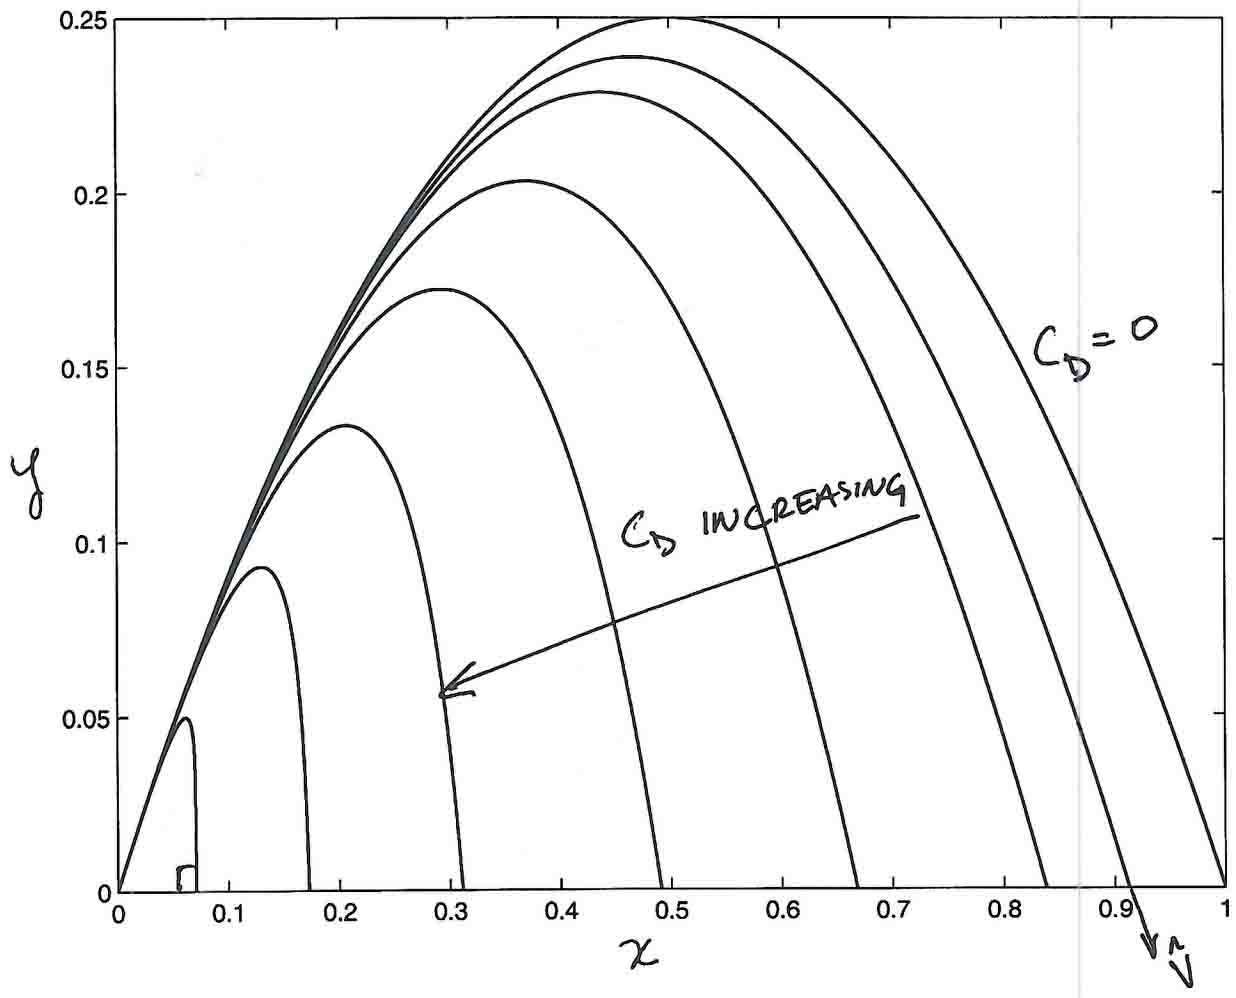
\includegraphics[width=5cm]{drag.jpg}
\end{example}


